\documentclass[preprint]{sig-alternate-05-2015}


\usepackage[utf8]{inputenc}
\usepackage[T1]{fontenc}
\usepackage{hyperref}
\usepackage{booktabs}
\usepackage{paralist}

\usepackage{enumerate}
\usepackage{subcaption}
\usepackage{cleveref}
\usepackage{ucs}
\usepackage{framed}

\usepackage[labelfont=bf]{caption}

\hypersetup{
    colorlinks,
    linkcolor={red!65!black},
    citecolor={blue!50!black},
    urlcolor={blue!80!black}
}

\usepackage{listings}  

\lstset{
language=PHP,
basicstyle=\small\sffamily,
numbers=left,
numberstyle=\tiny,
frame=tb,
columns=fullflexible,
showstringspaces=false
}

% ARIAL
%\usepackage{helvet}
%\renewcommand{\familydefault}{\sfdefault}


% TIMES
\usepackage{mathptmx}% http://ctan.org/pkg/mathptmx

\usepackage{pgfplots, pgfplotstable}

\usepackage{xcolor}

\definecolor{orange}{RGB}{230, 100, 20}
\definecolor{gruen}{RGB}{255, 190, 69}

\definecolor{RYB1}{HTML}{DCDCDC}
\definecolor{RYB2}{HTML}{C0C0C0}
\definecolor{RYB3}{HTML}{808080}

\definecolor{RYB4}{HTML}{DCDCDC}
\definecolor{RYB5}{HTML}{C0C0C0}
\definecolor{RYB6}{HTML}{808080}

\definecolor{RYB7}{HTML}{DCDCDC}
\definecolor{RYB8}{HTML}{C0C0C0}
\definecolor{RYB9}{HTML}{808080}

\definecolor{RYB10}{HTML}{D3D3D3}
\definecolor{RYB11}{HTML}{A9A9A9}

\pgfplotscreateplotcyclelist{ColorListBar}{
{fill=RYB1},
{fill=RYB2},
{fill=RYB3},
}

\pgfplotscreateplotcyclelist{ColorListBar2}{
{fill=RYB4},
{fill=RYB5},
{fill=RYB6},
}

\pgfplotscreateplotcyclelist{ColorListBar3}{
{fill=RYB7},
{fill=RYB8},
{fill=RYB9},
}

\begin{document}
\lstset{
	language=PHP,
	basicstyle=\footnotesize\ttfamily,
    commentstyle = \color{gray},
    extendedchars = \true,
    inputencoding = utf8x,
    keepspaces = true,
    keywordstyle = \bfseries
}

% Copyright
\setcopyright{acmcopyright}
%\setcopyright{acmlicensed}
%\setcopyright{rightsretained}
%\setcopyright{usgov}
%\setcopyright{usgovmixed}
%\setcopyright{cagov}
%\setcopyright{cagovmixed}


% DOI
\doi{10.475/123_4}

% ISBN
\isbn{123-4567-24-567/08/06}

%Conference
\conferenceinfo{ISSTA '17}{July 9--13, 2013, Santa Barbara, CA, USA}

\acmPrice{\$15.00}

%
% --- Author Metadata here ---
\conferenceinfo{ISSTA '17}{July 9--13, 2013, Santa Barbara, CA, USA}
%\CopyrightYear{2007} % Allows default copyright year (20XX) to be over-ridden - IF NEED BE.
%\crdata{0-12345-67-8/90/01}  % Allows default copyright data
% (0-89791-88-6/97/05) to be over-ridden - IF NEED BE.
% --- End of Author Metadata ---

\title{Does It Scale? Static Output Approximation of PHP Web Applications Using
Symbolic Execution} 

%


\numberofauthors{3} %  in this sample file, there are a *total*
% of EIGHT authors. SIX appear on the 'first-page' (for formatting
% reasons) and the remaining two appear in the \additionalauthors section.
%
\author{
% You can go ahead and credit any number of authors here,
% e.g. one 'row of three' or two rows (consisting of one row of three
% and a second row of one, two or three).
%
% The command \alignauthor (no curly braces needed) should
% precede each author name, affiliation/snail-mail address and
% e-mail address. Additionally, tag each line of
% affiliation/address with \affaddr, and tag the
% e-mail address with \email.
%
% 1st. author
\alignauthor
Stefan Mühlbauer\\
       \affaddr{TU Braunschweig, Germany}\\
       %\email{s.muehlbauer@tu-bs.de}
% 2nd. author
\alignauthor
Christian Kästner\\
      \affaddr{Carnegie Mellon University, USA}\\
       %\email{ckaestner@cs.cmu.edu}
% 3rd. author
\alignauthor
Tien N. Nguyen\\
       \affaddr{University of Texas, USA}\\
%      %\email{tien.n.nguyen@utdallas.edu}
}
% There's nothing stopping you putting the seventh, eighth, etc.
% author on the opening page (as the 'third row') but we ask,
% for aesthetic reasons that you place these 'additional authors'
% in the \additional authors block, viz.
\additionalauthors{Additional authors: John Smith (The Th{\o}rv{\"a}ld Group,
email: {\texttt{jsmith@affiliation.org}}) and Julius P.~Kumquat
(The Kumquat Consortium, email: {\texttt{jpkumquat@consortium.net}}).}
\date{30 July 1999}
% Just remember to make sure that the TOTAL number of authors
% is the number that will appear on the first page PLUS the
% number that will appear in the \additionalauthors section.

\maketitle
\begin{abstract}
Dynamic web applications have become widely popular and are to
a large proportion based on the scripting language PHP. Output approximation of web
applications enables a range of additional tool support as well as possibilities
for vulnerability detection. Unfortunately, recent approximation approaches have
only been evaluated for smaller systems.

This paper presents an experience report about the scalability of output
approximation using symbolic execution of state-of-the-art PHP web
applications. For a symbolic execution engine extended with support for
object-oriented programming and arrays, we identified language features and
corresponding programming patterns that impede symbolic execution and limit the
scalability of this approach. Our findings include: (1) Dynamic features such as
functions and includes are prone to fail for certain programming patterns. (2)
Expressions containing elements from I/O, databases or files can heavily impede
symbolic execution. Our findings provide useful guidelines to design new
tools and also to improve the development process of statically analyzable web
applications.
\end{abstract}


%
% The code below should be generated by the tool at
% http://dl.acm.org/ccs.cfm
% Please copy and paste the code instead of the example below. 
%
\begin{CCSXML}
<ccs2012>
 <concept>
  <concept_id>10010520.10010553.10010562</concept_id>
  <concept_desc>Computer systems organization~Embedded systems</concept_desc>
  <concept_significance>500</concept_significance>
 </concept>
 <concept>
  <concept_id>10010520.10010575.10010755</concept_id>
  <concept_desc>Computer systems organization~Redundancy</concept_desc>
  <concept_significance>300</concept_significance>
 </concept>
 <concept>
  <concept_id>10010520.10010553.10010554</concept_id>
  <concept_desc>Computer systems organization~Robotics</concept_desc>
  <concept_significance>100</concept_significance>
 </concept>
 <concept>
  <concept_id>10003033.10003083.10003095</concept_id>
  <concept_desc>Networks~Network reliability</concept_desc>
  <concept_significance>100</concept_significance>
 </concept>
</ccs2012>  
\end{CCSXML}

\ccsdesc[500]{Computer systems organization~Embedded systems}
\ccsdesc[300]{Computer systems organization~Redundancy}
\ccsdesc{Computer systems organization~Robotics}
\ccsdesc[100]{Networks~Network reliability}



%
%  Use this command to print the description
%
\printccsdesc

% We no longer use \terms command
%\terms{Theory}

\keywords{Static program behavior, Static metrics, Dynamic language features,
Static Analysis, PHP}

\section{Introduction}
With the emerge of the world wide web, dynamic web applications have become
widely popular. Various different implementation techniques have emerged,
ranging from technologies for programming languages (JSP, ASP .NET) and web
application frameworks for  script languages (Ruby On Rails, Django) to
languages tailored specifically to the domain of web applications. PHP \cite{phpNET} is
a programming language focused on server-side application development. As of 2012,
it was used by 78.8 percent of the ten million most popular websites (according
to Alexa popularity ranking) \cite{alexaPHP}, ranking 7th on the TIOBE
programming community index \cite{tiobePHP}, and was the ranked as the 6th most
popular language on GitHub \cite{githubPHP}.\\

One common property of all technologies for dynamic we b applications is the
\emph{staged computation} of output, or simplified: dynamic code generation.
Since based on both static values and runtime values, output code is generated step by step
dynamically, output can be dependent on application inputs. Dynamic web
applications incorporate various both server-side inputs (databases,
configuration) and client-side inputs respectively. Static
analysis of dynamic web applications, hence, has to consider different input
sources.

\emph{Symbolic execution} is a static analysis technique between program testing
and program proving. For a program, symbolic, i.e., abstract, yet fix inputs are
applied instead of concrete inputs \cite{Darringer1978,King1976}. The underlying
concept is to map program input (symbolically) to program output. Different classes of inputs may
result in variational output, representing dependencies of output and input.
Symbolic execution extends concrete execution semantics with semantics to
handle symbolic values. Hence, concrete execution semantics is contained in
symbolic execution semantics.\\

Symbolic execution has been used and studied for generating test suites, but
has more recently also been applied for approximating the output of web
applications. Knowledge about different output variants enabled useful analyses
for the domain of web applications, such as detecting and locating HTML
validation errors \cite{Nguyen:2011:AFH:2190078.2190142}. As for developers,
from an output model, outlines and callgraphs for easier IDE code navigation
\cite{Nguyen:2014:BCG:2635868.2635928}, or program slices
\cite{Nguyen:2015:CPS:2786805.2786872} can be computed. Existing work has been
integrated in the Varis plugin for the Eclipse IDE \cite{Nguyen:2015:VIS:2819009.2819140}.

Despite the various use cases for analyses based on an approximated output
model, static output approximation for PHP web applications using symbolic
execution has so far only been evaluated for smaller systems that are not
developed anymore. The previously mentioned tools though are only practical, if
for a given system the symbolic execution engine is scalable, i.e., will also
approximate reliable output for larger and more recent systems with good time
and space consumption.\\

To investigate the question, whether we can have practical tools built from the
symbolic execution engine, we re-implemented the engine with the specifications
of the previous symbolic execution semantics
\cite{Nguyen:2014:BCG:2635868.2635928} for PHP and additional features, such as
object-oriented programming, and extensive array support. We evaluated our
symbolic execution engine for large-scale and modern PHP systems.

During introduction of new semantics for object-orientation and advanced array
we encountered two main challenges. First, we walked a boundary between a
purely symbolic or mixed concrete and symbolic (concolic) execution engine
since concrete execution, e.g. foreach loops for arrays, increased code
coverage significantly. Second, we had to make a trade-off between the accuracy
of method calls and the scalability of this language feature as a method call
for different program state variants can have multiple targets.

Based on our observations and evaluation results, we learned that for dynamic
PHP constructs, expressions that are assembled dynamically, in combination with
symbolic values symbolic execution can be impractical. For object-orientation
and method calls, symbolic execution semantics can be a tightrope walk between
state space explosion and imprecision. Moreover, the nature of PHP challenges a
practical symbolic execution engine since for it to be accurate, a large number
of functions from the standard library needs to be supported.\\

Our key contributions in this paper include: (1) The tool infrastructure to
statically approximate the output for PHP web applications using symbolic
execution and (2) observations as well as an experience evaluation to identify
and measure PHP constructs impeding symbolic execution of PHP code.

\section{State Of the Art}

\section{Towards scalable symbolic execution}%


\section{Evaluation}
As already stated in the previous section, we encountered sevaral problems
during the development of the symbolic interpreter. Therefore this section
describes our methods to evaluate practicality of the output approximation, and
possible explanations.

\subsection{Measuring Approximation Success} \label{heuristic}
For the evaluation of our output approximation we require a ground truth output model to compare against.
In the absence of ground truth for the approximated output we are bound to choose a \emph{heuristic approach} in order to measure the accuracy of our aproximation. We define a string literal to be an \emph{output candidate} if there exists an execution path reaching the string literal and evantually passing it to an 
output-generating statement (e.g., \texttt{echo} or \texttt{print}).

We approximate output candidates as those string literals containing the characters \texttt{<}, \texttt{>}, or both since we expect output to contain HTML tags. We evaluated this heuristic manually
with a sample of 400 string literals randomly selected from the entire corpus.
We measured for our heuristic classifier a precision of 94 percent, and a recall
of 50 percent. This means that six percent of the string literals are classified incorrectly as false positives. In turn, the classifier is highly distinctive as 96 percent of the string literals are classified correctly. The recall of 50 percent means that half of the string literals, which we manually classified as output, actually were responsive to the classifier. We attempted to increase recall by looking for further distinctive properties to build a classifier from, but could not do so without decreasing precision. In spite of missing half of the output candidates, we decided to use a simple, yet distinctive classifier.

\subsection{Experiment Setup} 
For the evaluation we symbolically executed a selection of PHP systems. We selected a corpus of twelve PHP systems with regard to system size and recency as the corpus of the case study for \cite{Nguyen:2014:BCG:2635868.2635928} only contained small-scale systems that are not maintained any more. The full list of PHP systems is shown in Table \ref{corpus}. Our selection of PHP systems includes
%\begin{enumerate}[a)]
\begin{compactitem}
\item four small-scale systems that selected from the previously mentioned case study in order to compare our results with the previous symbolic execution engine \cite{Nguyen:2014:BCG:2635868.2635928},
\item three recent large-scale systems selected from the case study corpus of \cite{Hills:2013:ESP:2483760.2483786}, and
\item four small-scale systems selected from a list of recent Content Management Systems \cite{codegeekz}.
%umerate}

\end{compactitem}
As for for the last two cases, we limited our selection since the parser we
used did not support all language features used.

\begin{table*}[t]
\centering 
	\begin{tabular}{p{4cm}rrrl}
	\toprule
	\textbf{System} & \textbf{Version} & \textbf{File Count} & \textbf{SLOC} &
	\textbf{Description}
	\\
	\midrule
	AddressBook & 8.2.5.2 & 239 & 51,907 & Adress Administration \\
	SchoolMate & 1.5.4 & 65 & 8,118 & School Administration \\
	TimeClock & 1.04 & 63 & 20,800 & XXX \\
	WebChess & 1.0.0 & 28 & 5,219 & XXX \\
	\midrule
	Drupal & 7.5.0 & 125 & 52,464 & Content Management System \\
	phpBB & 3.1.9 & 1,398 & 327,371 & Bulletin Board \\
	phpMyAdmin & 4.6.3 & 871 & 303,582 & Database Administration \\
	\midrule
	Anchor & 0.12.1 & 201 & 15,054 & Content Management System \\
	Kirby & XXX & XXX & XXX & Content Management System \\
	Automad & XXX & XXX & XXX & Content Management System \\
	Monstra & XXX & XXX & XXX & Content Management System \\
	Nibbleblog & XXX & XXX & XXX & Content Management System \\
	\bottomrule
	\end{tabular}
	\caption{Corpus of twelve PHP systems. The file count includes files with a .php,
	.inc, .bit or .module extension.}
	\label{corpus}
\end{table*}

For the experimental analysis we symbolically executed per system each script file or entry point (files with a \texttt{.php}, \texttt{.inc}, \texttt{.bit} or \texttt{.module} extension). All following measurements are cumulated per system for each entry point. 

\subsection{Measuring Approximation Accuracy}
\label{HowAccurateIsOurApproximation} 
In Section \ref{heuristic} we introduced the definition of output candidates as expected output. As a most accurate approximation contains all output candidates, we define two metrics to measure accuracy of our approximation. 

First, we measure how much of the expected output was actually processed by the symbolic interpreter.  Once a line of code, a statement or expression containing an output candidate is actually an element in an execution path, we define this output candidate as reached. We define the metric \emph{reach coverage} as the ratio of output candidates that are reached and the total number of output candidates in the analyzed system. Although a reached output candidate is processed by the symbolic interpreter, it does not guarantee we will see that output candidate in the symbolic output. Second, we define the metric \emph{output coverage} as the ratio of output candidates that are contained in the output of the symbolic interpreter and the total number of output candidates in the analyzed system.  For an imprecise approximation, we may see loss of output candidate information resulting in a output coverage lower than the reach coverage.

The coverage results are illustrated in Figure \ref{coverage}. We could replicate high coverage results for the four small-scale systems with a reach coverage and output coverage over 80 percent respectively. For the three modern/large-scale systems we measured poor coverage with reach coverage ranging from 5 to 30 percent and output coverage ranging from 4 to 20 percent. We measured medium to high coverage for the more recent small-scale systems: reach coverage ranging from 43 to 85 percent, output coverage ranging from 40 to 85 percent.
% RESULTS
% REACH COVERAGE and
% OUTPUT COVERAGE
\begin{figure}
	\centering	
	\resizebox{0.4\textwidth}{!}{%
		\pgfplotstableread[header=false, col sep=comma]{ 
	86.32, AdressBook
	100.0, SchoolMate
	92.36, TimeClock
	91.28, WebChess
	31.44, phpBB
	19.99, Drupal
	5.000, phpMyAdmin
	90.48, Anchor
	76.3,  Kirby
	46.87, Automad
	79.47, Monstra
	71.37, Nibbleblog
	}\datatablex
	
	\pgfplotstableread[header=false, col sep=comma]{ 
	84.44, AdressBook
	98.24, SchoolMate
	91.22, TimeClock
	88.72, WebChess
	4.76, phpBB
	18.39, Drupal
	3.79, phpMyAdmin
	89.56, Anchor
	76.30,  Kirby
	40.15, Automad
	61.38, Monstra
	59.43, Nibbleblog
	}\datatable
	
	\begin{tikzpicture}[thick,scale=0.8, every node/.style={transform shape}]
	  \begin{axis}[   
	  	,legend style={at={(0.25,-0.2)},
		anchor=north,legend columns=-1} 
	    ,xbar
	    ,xlabel={Coverage [\%]}
	    ,bar width=1ex, y=3ex
	    ,enlarge y limits={abs=0.75}
	    ,ytick={data} % (\empty,data,{coordinate list})
	    ,label={Reach}
	    ,yticklabels from table={\datatable}{1}
	  ]
	  
	  \addplot[red!20!black,fill=gray!80!white] table [
	    y expr=-\coordindex, % Use negative coordinate index as y coordinate
	    x index=0 % Use first column as x coordinate
	  ] {\datatable};
	  \addplot[red!20!black,fill=RYB2!100!white] table [
	    y expr=-\coordindex, % Use negative coordinate index as y coordinate
	    x index=0 % Use first column as x coordinate
	  ] {\datatablex};
	  
	  \legend{Output, Reached}
	  \end{axis}
	\end{tikzpicture}	
	}
	\caption{Coverage results for the PHP corpus}
	\label{coverage}
\end{figure}

\subsection{Understanding Limitations}
As we have seen in Section \ref{HowAccurateIsOurApproximation} both measured coverage metrics were poor for large-scale and small-scale/recent systems. To understand what output candidates we missed and why, we further investigated our approximation results and conducted three more measurements. 

\subsubsection{What literals did we miss?}
\label{WhatLiteralsDidWeMiss?}
Our initial approach to understand missed output candidates is to find out whether their surrounding program code was not accessed/accessible, and if so, why. Of special interest are those output candidates that are located in HTML files (possibly with nested PHP), or located in a function definition. Plain HTML files do not require any further execution (of course, unless PHP scripts are embedded) and represent output candidates that just need to be included properly to be part of the output. Aside, output candidates that are part of a function definition are only missed if the corresponding function is never called at runtime.

We started classifying missed output candidates by their string literal context. As the classification statistics in Figure \ref{fig:contexts} illustrate, for almost all systems (except for \textsc{AddressBook} and \textsc{TimeClock}) not-reached output candidates had a function context. Note that \textsc{SchoolMate} was excluded from the diagram since our analysis reached all output candidates for that system.

% CONTEXT DISTRIBUTION
% - FUNCTION CONTEXT
% - TEMPLATE CONTEXT
\begin{figure}
	\resizebox{0.4\textwidth}{!}{%
		    \pgfplotstableread{ % data 
Label     Reached/Output OnlyReached FunctionContext Bener
Adressbook 3 2 1.4 3
Schoolmate 3 2 1 2
Timeclock 3 2 1 2
Webchess 3 2 1 2
PhpBB 3 2 1 2
Drupal 3 2 1 2
phpMyAdmin 3 2 1 2
Anchor 3 2 1 2
Kirby 3 2 1 2
Automad 3 2 1 2
Monstra 3 2 1 2
Nibbleblog 3 2 1 2
    }\testdata

    \begin{tikzpicture}[thick,scale=0.8, every node/.style={transform shape}]

    \begin{axis}[
    enlargelimits=0.05,
    xbar stacked,   % Stacked horizontal bars
    xlabel={Proportion [\%]},
    xmin=0,         % Start x axis at 0
    ytick=data,     % Use as many tick labels as y coordinates
    legend style={
       at={(0.5,-0.28)}, 
       anchor=north,
       legend columns = -1,
       cells={anchor=center, fill},
       nodes={inner sep=1,below=-1.1ex}
    },
    yticklabels from table={\testdata}{Label}  % Get the labels from the Label column of the \datatable
    ,bar width=2ex, y=3ex,
    nodes near coords = {%
       \pgfmathprintnumberto[fixed,assume math mode=true]{\pgfplotspointmeta}{\myval}%
       \pgfmathparse{\myval<101?:}\pgfmathresult%
    },
    area legend
    ]
    \addplot [fill=lightgrey!80] table [x=Reached/Output, meta=Label,y expr=\coordindex] {\testdata};
    \addplot [fill=blue!60] table [x=OnlyReached, meta=Label,y expr=\coordindex] {\testdata};
    \addplot [fill=red!60] table [x=FunctionContext, meta=Label,y expr=\coordindex] {\testdata};
    \addplot [fill=red!99] table [x=Bener, meta=Label,y expr=\coordindex] {\testdata};    
    
    \legend{Reached/Output, OnlyReached, FunctionContext, Bener}
    \end{axis}
    \end{tikzpicture}
	}	
	\caption{Context distribution of never reached output candidates for the PHP
	corpus.}
	\label{fig:contexts}
\end{figure}

\subsubsection{Inaccessible Dynamic Features}
\label{sec:inaccessible}
For both cases of context, either inclusion of a script file failed, or a function call failed. If an HTML file is not part of the output, it also is never reached, i.e., included. An include can fail due to various reasons, such as an imprecise evaluation of the include expression returning a symbolic value, or simply a missing file. 

For a function to be never reached there are several scenarios: A function is undefined at runtime if the corresponding script file is never included. In turn, if the function is defined at runtime the function can either be dead code if there is no call site for this function, or the function call failed. In PHP there are several ways to call a function beside direct call sites. The language offers indirect call mechanisms like callback-commands or an evaluation function that parses and evaluates PHP source code as strings.

Given a symbolic value, indirect call mechanisms like callback-commands are likely to fail since target function name and the symbolic value do not match. This also applies for the evaluation of include expressions as concrete values representing include targets can be included, but any include target containing symbolic values is ambiguous.

\subsubsection{Why did includes fail?}
\label{WhyDidIncludesFail}
To better understand include expression evaluation, we use another metric to approach accuracy from a different angle: We measure (1) the ratio of reached include expressions and the total number of include expressions in a system respectively (coverage of include expressions), and (2) the ratio of successfully resolved include expressions and reached include expressions in a system (resolution success rate). For a most accurate result all include expressions are reached and resolved.

For include expressions we sampled failed attempts and manually evaluated the cause of failure. We identified for (1) that all failed attempts were dynamic include expressions, i.e., those which were resolved at runtime and were assembled from fragments of environment-dependent information including database retrievals, user input, or files. Consequently, the resolved include expressions contained symbolic values which did not represent identifiable script files.

Finally, we measured for include expressions the overall reach coverage and the overall resolution success rate per system. As illustrated in Figure \ref{fig:include_coverage_results2}, except for the small-scale systems and two recent small-scale systems we did not even really reach a great portion of include expressions, although for most systems the resolution success rate was over 80 percent (see Figure \ref{fig:include_coverage_results1}). Nevertheless, one failed attempt to include a script file can result in a cascade of missing more include expressions as the include target script is not executed.

% INCLUDE COVERAGE / SUCCESS RATE
\begin{figure*}[t!]
    \centering
    \begin{subfigure}[t]{0.5 \textwidth}    	
        \centering        
        % Include Coverage Plot        
		        \pgfplotstableread[header=false, col sep=comma]{ 
		96.77, AdressBook
		100, SchoolMate
		92.48, TimeClock
		94.64, WebChess
		65.42, phpBB
		49.03, Drupal
		39.75, phpMyAdmin
		84.38, Anchor
		39.13,  Kirby
		37.5, Automad
		37.5, Monstra
		100, Nibbleblog
		}\reachedincludes
	
		\begin{tikzpicture}[thick,scale=0.8, every node/.style={transform shape}]
		  \begin{axis}[   
		  	,legend style={at={(0.25,-0.2)},
			anchor=north,legend columns=-1} 
		    ,xbar
		    ,xlabel={Reached include expressions [\%]}
		    ,bar width=1.2ex, y=2ex
		    ,enlarge y limits={abs=0.75}
		    ,ytick={data} % (\empty,data,{coordinate list})
		    ,label={Reach}
		    ,yticklabels from table={\reachedincludes}{1}
		  ]
		  
		  \addplot[red!20!black,fill=RYB10!80!white] table [
		    y expr=-\coordindex, % Use negative coordinate index as y coordinate
		    x index=0 % Use first column as x coordinate
		  ] {\reachedincludes};
		  
		  \end{axis}
		\end{tikzpicture}		
        \caption{Proportion of reached include expressions per project.}
        \label{fig:include_coverage_results1}
    \end{subfigure}%
	\hfill
    \begin{subfigure}[t]{0.5\textwidth}    
        \centering
        % Success Rate Plot        
        \pgfplotstableread[header=false, col sep=comma]{ 
		95, AdressBook
		100, SchoolMate
		100, TimeClock
		100, WebChess
		74, phpBB
		88, Drupal
		99, phpMyAdmin
		0, Anchor
		0,  Kirby
		100, Automad
		27, Monstra
		90, Nibbleblog
		}\successfulincludes
	
		\begin{tikzpicture}[thick,scale=0.8, every node/.style={transform shape}]
		  \begin{axis}[   
		  	,legend style={at={(0.25,-0.2)},
			anchor=north,legend columns=-1} 
		    ,xbar
		    ,xlabel={Successfully resolved and reached include expressions [\%]}
		    ,bar width=1.2ex, y=2ex
		    ,enlarge y limits={abs=0.75}
		    ,ytick={data} % (\empty,data,{coordinate list})
		    ,label={Reach}
		    ,yticklabels from table={\successfulincludes}{1}
		  ]
		  
		  \addplot[red!20!black,fill=RYB11!80!white] table [
		    y expr=-\coordindex, % Use negative coordinate index as y coordinate
		    x index=0 % Use first column as x coordinate
		  ] {\successfulincludes};
		  
		  \end{axis}
		\end{tikzpicture}        
        \caption{Rate of successful resolutions of reached include expressions
        per project.}
        \label{fig:include_coverage_results2}
    \end{subfigure}
    \label{fig:include_coverage_results}
    \caption{Include coverage and accuracy.}
\end{figure*}

\subsubsection{Why did function calls fail?}
\label{WhyDidFunctionCallsFail}
Aside from failed or successful includes, this metric describes one scenario of why functions containing not-reached output candidates are never called: The trivial explanation would be that there are no direct calls of those functions, yet PHP offers a number of ways to call a function indirectly, for instance using built-in functions, or simply evaluating strings as PHP code using the \texttt{eval} function. 

Moreover we need to take into account that one missed function execution can result in missing even more function calls (direct or indirect) and executions. Thus, for functions containing not-reached output candidates we measure whether they can be (1) only, (2) partially or (3) never accessed transitively from functions that have no direct call sites. We refer to those functions (or access points) having no direct call site as callback candidates since the only way to reach them is through indirect mechanisms. Measuring how many not-reached output candidates can be explained by functions that are callback candidates helps to understand whether, and if so, indirect call mechanisms and their usage may impact our analysis’ code coverage.

The callgraph snippets in Figure \ref{fig:callgraph} illustrate the idea of detecting the functions’ access points: The nodes at the top depict callback candidates, the nodes at the bottom with labels X, Y, and Z depict function definitions containing not-reached output candidates. In Figure \ref{fig:callgraph_a} function X can only be accessed through callback candidates, as for Figure \ref{fig:callgraph_b} function Y can be partially accessed by callback candidates, whereas function Z is never accessible through callback candidates.

% Callback candidate description
\begin{figure}
	\centering
	\begin{subfigure}[t]{0.18\textwidth}
	\centering
		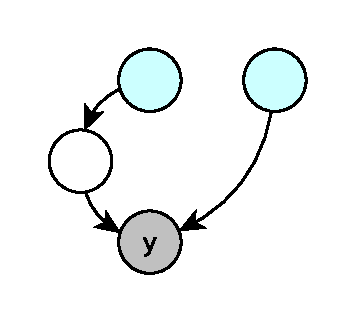
\includegraphics[scale=0.4]{images-paper/callgraph_a}
		\caption{Completely explained by callback candidates (no call from
		\texttt{main})}
		\label{fig:callgraph_a}
    \end{subfigure}
	\hfill
	\begin{subfigure}[t]{0.25\textwidth}
	\centering
		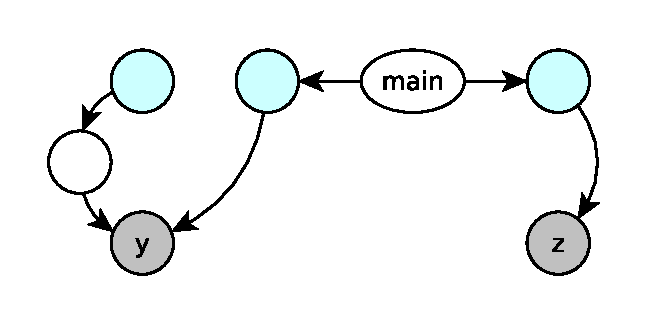
\includegraphics[scale=0.4]{images-paper/callgraph_b}
		\caption{Partially (left; one call from \texttt{main}) or not at all  (right)
		explained by callback candidates}
		\label{fig:callgraph_b}
    \end{subfigure}
    \caption{Callgraph analysis: The bottom nodes represent functions containing missed output candidates, the top nodes depict entry points to them.}
    \label{fig:callgraph}
\end{figure}

Like for include expressions, we again sampled dead function cases and identified the lack of direct call sites to those functions. As described in Section \ref{sec:inaccessible}, functions despite having no direct call sites were called through indirect call features. We identified dynamically assembled expressions (function names) to be responsible for failed attempts of calling a function indirectly as the resolved function name eventually contained symbolic values. These expressions, as well as include expressions, contained information dependent on the system environment.

For failed function calls to functions containing not-reached output candidates we measured how many of those functions were only, or partially accessibly through indirect calling mechanisms (see Section \ref{sec:inaccessible}). As Figure \ref{fig:output_candidate_explanation} illustrates, around 80 percent (except for \textsc{TimeClock}) all missed output candidates of each system were only accessible through callback candidates, i.e., functions that are only accessible through indirect calling mechanisms.

% CALLBACK CANDIDATE ACCESSIBILITY ANALYSIS
\begin{figure}[p]
	\begin{tikzpicture}[thick,scale=0.8, every node/.style={transform shape}]
\begin{axis}[
    ybar stacked,
	bar width=12pt,
	nodes near coords = {%
    \pgfmathprintnumberto[fixed,assume math mode=true]{\pgfplotspointmeta}{\myval}%
    \pgfmathparse{\myval<101?:\myval}\pgfmathresult%
},
    enlargelimits=0.15,
    legend style={at={(0.5,-0.28)},
      anchor=north,legend columns=-1},
    ylabel={Proportion [\%]},
    symbolic x coords={AddressBook, TimelClock, WebChess, Drupal,
    phpBB, phpMyAdmin, Anchor, Kirby, Automad, Monstra, Nibbleblog}, xtick=data,
    x tick label style={rotate=45,anchor=east},
    cycle list name=ColorListBar3,
    ]

\addplot+[ybar] plot coordinates {(AddressBook, 100) 
  (TimelClock, 0) (WebChess, 79) (Drupal, 87) (phpBB, 94) (phpMyAdmin, 99)
  (Anchor, 79) (Kirby, 98) (Automad, 100) (Monstra, 100) (Nibbleblog, 100)};
\addplot+[ybar] plot coordinates {(AddressBook, 0) 
  (TimelClock, 0) (WebChess, 0) (Drupal, 3) (phpBB, 1) (phpMyAdmin, 0)
  (Anchor, 3) (Kirby, 1) (Automad, 0) (Monstra, 0) (Nibbleblog, 0)};
\addplot+[ybar] plot coordinates {(AddressBook, 0) 
  (TimelClock, 100) (WebChess, 21) (Drupal, 10) (phpBB, 5) (phpMyAdmin, 0)
  (Anchor, 18) (Kirby, 1) (Automad, 0) (Monstra, 0) (Nibbleblog, 0)};

\legend{Complete, Partial, None}
\end{axis}
%\caption{Relative distribution of contexts of not reached output candidates}
\end{tikzpicture}
	\caption{Distribution dead function output candidates that are partially or
	completely explained due to callback candidates.}
	\label{fig:output_candidate_explanation}
\end{figure}



\section{Lessons Learned}

		\begin{lstlisting}[caption=A misplaced and unused \texttt{listing} with no real value to this paper.]
		function foo() {
   		   echo "foo";
		}
		\end{lstlisting}


\section{Related Work}

%References
\bibliographystyle{abbrv}
\bibliography{bibliography}

\end{document}
